
\de{ĐỀ THI HỌC KỲ I NĂM HỌC 2022-2023}{THPT Nguyễn Thượng Hiền}


\begin{bt}%[0T1B2-1]%[Dự án đề kiểm tra HKII NH22-23- Nguyễn Ngọc Nguyên]%[THPT Nguyễn Thượng Hiền]
	Cho tập hợp $A=\{x\in \mathbb{N}\Big|(x-1)(x^2-x-2)=0\}$. Viết tập hợp $A$ dưới dạng liệt kê các phần tử và viết tất cả các tập hợp con của tập hợp $A$.
\loigiai{
Ta giải phương trình 
\begin{eqnarray*}
	(x-1)(x^2-x-2)=0 \Leftrightarrow \hoac{&x-1=0 \\ & x^2-x-2=0} \Leftrightarrow \hoac{&x=1 \\ &x=-1 \\ &x=2.}
\end{eqnarray*}
Mà $x \in \mathbb{N}$ nên $x=1$, $x=2$.\\
Vậy $A= \{1;2\}$ và các tập con của $A$ là $\{1\}$, $\{2\}$, $\{1;2\}$ và $\varnothing$.
}
\end{bt}

\begin{bt}%[0T3B1-2]%[Dự án đề kiểm tra HKII NH22-23- Nguyễn Ngọc Nguyên]%[THPT Nguyễn Thượng Hiền]
Tìm tập xác định của hàm số $f(x)=\dfrac{\sqrt{x+1}+\sqrt{4-x}}{-x^2-2x+3}$.
\loigiai{
Điều kiện xác định
\begin{eqnarray*}
	\heva{& x+1 \ge 0 \\ &4-x \ge 0 \\ &-x^2-2x+3 \ne 0} \Leftrightarrow \heva{&x \ge -1 \\ & x \le 4 \\ & x \ne 1 \\ & x \ne -3} \Leftrightarrow \heva{& -1 \le x \le 4 \\ & x \ne 1.}
\end{eqnarray*}	
Vậy tập xác định là $\mathscr{D}=[-1;4]\setminus\{1\}$.}
\end{bt}


\begin{bt}%[0T3B1-3]%[0T3B1-4]%[Dự án đề kiểm tra HKII NH22-23- Nguyễn Ngọc Nguyên]%[THPT Nguyễn Thượng Hiền]
	\immini{Cho hàm số xác định trên đoạn $[-3;2]$ như hình bên, hãy xác định các khoảng biến thiên và tập giá trị của hàm số đó trên đoạn $[-3;2]$.}{
	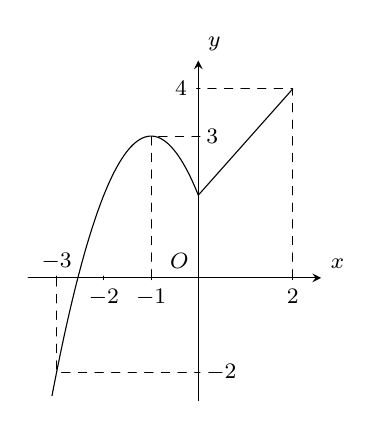
\begin{tikzpicture}[scale=1, font=\footnotesize, line join=round, line cap=round, >=stealth]
		\begin{scope}[scale=.6]
			\draw[->] (-3.6,0)--(2.6,0) node[above right] {$x$};
			\draw[->] (0,-2.6)--(0,4.6) node[above right] {$y$};
			\draw (0,0) node [above left] {$O$};
			\foreach \x in {-2,-1,2}
			\draw[thin] (\x,1pt)--(\x,-1pt) node [below] {$\x$};
			\foreach \x in {-3}
			\draw[thin] (\x,1pt)--(\x,-1pt) node [above] {$\x$};
			\foreach \y in {-2,3}
			\draw[thin] (1pt,\y)--(-1pt,\y) node [right] {$\y$};
			\foreach \y in {4}
			\draw[thin] (1pt,\y)--(-1pt,\y) node [left] {$\y$};
			\draw[dashed,thin](-1,0)--(-1,3)--(0,3);
			\draw[dashed,thin](-3,0)--(-3,-2)--(0,-2);
			\draw (0,7/4)--(2,4);
			\draw[dashed,thin] (2,0)--(2,4)--(0,4);
			\begin{scope}
				\clip (-3.5,-2.5) rectangle (2.5,4.5);
				\draw[samples=200,domain=-3.5:0,smooth,variable=\x] plot (\x,{-5/4*(\x)^2+-5/2*(\x)+7/4});
			\end{scope}
		\end{scope}
	\end{tikzpicture}
}
\loigiai{
Đồ thị hàm số đi lên trong các khoảng $(-3;-1)$ và $(0;2)$ nên hàm số đồng biến trên khoảng $(-3;-1)$ và $(0;2)$.\\
Đồ thị hàm số đi xuống trong khoảng	$(-1,0)$ nên hàm số nghịch biến trên khoảng $(-1,0)$.\\
Điểm thấp nhất nằm trên đồ thị hàm số trong đoạn $[-3;2]$ có tung độ là $-2$. \\
Điểm cao nhất nằm trên đồ thị hàm số trong đoạn $[-3;2]$ có tung độ là $4$.\\
Do đó tập giá trị của hàm số trên đoạn $[-3;2]$ là $T=[-2;4]$.}
\end{bt}


\begin{bt}%[0T3K2-2]%[Dự án đề kiểm tra HKII NH22-23- Nguyễn Ngọc Nguyên]%[THPT Nguyễn Thượng Hiền]
Cho hàm số bậc hai $y=ax^2+bx+c$ ($a\ne 0)$ có đồ thị là parabol $(P)$. Biết rằng $(P)$ có đỉnh $I(1;3)$ và cắt trục tung tại điểm có tung độ là $4$. Xác định $a$, $b$, $c$.
\loigiai{
Vì hoành độ đỉnh $I$ của parabol là $1$ nên ta có $\dfrac{-b}{2a}=1 \Leftrightarrow 2a+b=0$. \tagEX{1}
\noindent Vì $I(1;3) \in (P)$ nên $a+b+c=3$. \tagEX{2}
\noindent Vì $(P)$ cắt $Oy$ tại điểm có tung độ bằng $4$ nên $c=4$.  \tagEX{3}
\noindent Từ $(1)$, $(2)$, $(3)$ ta có
\begin{eqnarray*}
	\heva{&2a+b=0 \\ & a+b+c=3 \\ & c=4} \Leftrightarrow \heva{&a=1 \\&b=-2 \\ & c=4.}
\end{eqnarray*}
Vậy $a=1$, $b=-2$, $c=4$.
}
\end{bt}


\begin{bt}%[0T6B3-1]%[0T6B4-2]%[Dự án đề kiểm tra HKII NH22-23- Nguyễn Ngọc Nguyên]%[THPT Nguyễn Thượng Hiền]
	Kết quả điểm thi GHK1 môn Toán của lớp $10A$ được cho bởi bảng sau
	\begin{center}
		\begin{longtable}{|c|c|c|c|c|c|c|}
			\hline
			Điểm & $5$ & $6$ & $7$ & $8$ & $9$ & $10$\\
			\hline
			Số lượng & $2$& $5$ & $9$ & $12$ & $10$ & $2$\\
			\hline
		\end{longtable}
	\end{center}
	Tìm số điểm trung bình môn Toán của lớp $10A$. Xác định độ lệch chuẩn của mẫu số liệu trên và nêu ý nghĩa của nó.
\loigiai{
Điểm trung bình của lớp là
\begin{eqnarray*}
	\overline{x}=\dfrac{5 \cdot 2 + 6 \cdot 5 + 7 \cdot 9 + 8 \cdot 12 + 9 \cdot 10 + 10 \cdot 2}{40}=7{,}725.
\end{eqnarray*}
Độ lệch chuẩn của mẫu số liệu là
\begin{eqnarray*}
	S=\sqrt{\dfrac{2(5-\overline{x})^2+5(6-\overline{x})^2+9(7-\overline{x})^2+12(8-\overline{x})^2+10(9-\overline{x})^2+2(10-\overline{x})^2}{40}} \approx 1{,}2447.
\end{eqnarray*}
Độ lệch chuẩn $S\approx 1{,}2447$ ở mức thấp, cho thấy mức độ chênh lệch điểm thi GHK1 môn Toán không đáng kể.
}
\end{bt}


\begin{bt}%[0T5B2-5]%[Dự án đề kiểm tra HKII NH22-23- Nguyễn Ngọc Nguyên]%[THPT Nguyễn Thượng Hiền]
	\immini{Một máy bay có véc-tơ vận tốc chỉ theo hướng bắc, vận tốc gió là một véc-tơ theo hướng đông như hình bên. Tính độ dài véc-tơ tổng của hai véc-tơ nói trên.}{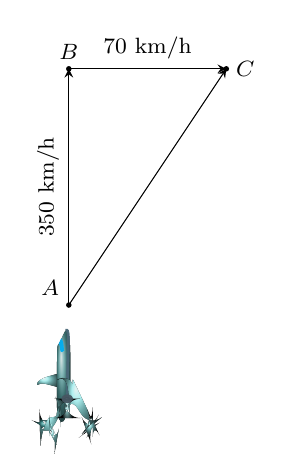
\begin{tikzpicture}[scale=1, font=\footnotesize, line join=round, line cap=round, >=stealth]
			\tikzset{
				maybay/.pic={
					\begin{scope}[line width=1pt,opacity=0.95]
						\fill[ball color =cyan!40!gray,,rounded corners=2mm](-5.6,3)--++(60:0.8)--++(2:0.55)--++(-90:2)--cycle;
						%Hai cánh
						\fill[ball color =cyan!90!gray!40!white](-0.4,1.5)..controls++(75:2)and++(-68:0.75)..(-0.15,4)--++(-5:0.35)..controls++(-50:0.95)and++(106:2)..(1.25,1.5)--cycle;
						%Thân
						\fill[ball color =cyan!30!gray](-4.85,1)..controls++(-90:0.6) and++(180:0.2)..(-4,0.5)--++(-12:3.3)--++(0:4)..controls++(0:2) and++(-172:1)..(6,0)..controls++(8:1)and++(-90:0.1)..(6.85,0.3)..controls++(90:0.2) and++(-30:1)..(5,1.3)..controls++(90:0.25) and++(0:8)..(-4,1.5)--cycle;
						\draw[cyan!40!black](6.85,0.3)..controls++(-90:0.5) and++(0:6)..(-2,0.2);
						% Cánh phải
						\fill[ball color =cyan!90!gray!40!white,rounded corners=2mm](-1.8,0)--++(-5:0.35)--++(-147:4.85)--++(-50:0.7)--++(25.5:6.5)..controls++(-155.5:0.5) and++(-170:0.15)..(1.5,-0.25)..controls++(120:0.5) and++(2:1)..(-1.8,0);
						\fill[ball color =cyan!90!gray!40!white,rounded corners=2mm](-6.1,-2.3)--++(-54:0.7)--++(-28:0.7)--++(25.5:.35)--++(-180:.2)--++(135:1.2)--cycle;
						%Thân đuôi
						\fill[ball color =cyan!90!gray!40!white,rounded corners=2mm](-6.9,3.6)--++(2:1)..controls++(-35:2) and++(178:2.3)..(-2,1.5)..controls++(-90:0.2) and++(20:1)..(-3.5,1)--++(180:1.2)--cycle;
						%Đuôi
						\fill[ball color =cyan!90!gray!40!white,rounded corners=2mm](-6,2.5)--++(0:1.35)--++(-156:2.5)--++(170:0.75)--cycle;
						\fill[ball color =cyan!70!gray!40!white,rounded corners=2mm](-1.9,-0.17)--++(90:0.72)--++(181:2.45)--++(-90:0.6)--cycle;
						\fill[ball color =cyan!90!gray!10!black,line width=2pt,draw=cyan!30!black,rounded corners=0.5mm](-1.9,-0.18)arc(-90:270:0.2 and 0.38);
						\fill[cyan](5.05,1.3)--++(-25:0.8)..controls++(-140:0.55)and++(10:0.5)..(4.2,0.6)..controls++(180:0.15) and++(182:0.45)..(4.3,1.1)..controls++(2:0.5) and++(-135:0.2)..(5.1,1.3);
					\end{scope}
				}
			}
			\path (0,0) coordinate (O) pic[rotate=90,scale=.1]{maybay} 
			(O)+(90:1) coordinate (A)
			++(90:4) coordinate (B)
			++(0:2) coordinate (C)
			;
			\path[fill=black] (A) circle(1pt) node[above left]{$A$}
			(B) circle (1pt) node[above] {$B$}
			(C) circle (1pt) node[right]{$C$}
			;
			\draw[->] (A)--(B) node [midway,above,sloped] {$350$ km/h};
			\draw[->] (B)--(C) node [midway,above,sloped] {$70$ km/h};
			\draw[->] (A)--(C);
	\end{tikzpicture}}
\loigiai{
Ta có $\overrightarrow{AB}+\overrightarrow{BC}=\overrightarrow{AC}$.\\
Do đó độ dài của véc-tơ tổng chính là độ dài véc-tơ $\overrightarrow{AC}$.\\
Tam giác $ABC$ vuông tại $B$, theo định lý Py-ta-go ra có $AC=\sqrt{AB^2+BC^2}=\sqrt{350^2+70^2}=70\sqrt{26}$.\\
Vậy độ dài véc-tơ tổng cần tìm là $70\sqrt{26}$ km/h.}
\end{bt}


\begin{bt}%[0T5K3-2]%[Dự án đề kiểm tra HKII NH22-23- Nguyễn Ngọc Nguyên]%[THPT Nguyễn Thượng Hiền]
	Cho tam giác $ABC$ có $M$ là trung điểm của đoạn $AB$, điểm $N$ thuộc cạnh $AC$ sao cho $NC=2NA$ và gọi $K$ là trung điểm của $MN$. Chứng minh rằng $\vec{AK}=\dfrac{1}{4}\vec{AB}+\dfrac{1}{6}\vec{AC}$.
	\loigiai{
\immini{Ta có $M$ là trung điểm $AB$ nên $\overrightarrow{AM}=\dfrac{1}{2}\overrightarrow{AB}$.\\
Ta cũng có $NC=2NA$ nên $\dfrac{NC}{NA}=2 \Leftrightarrow \overrightarrow{AN}=\dfrac{1}{3}\overrightarrow{AC}$.\\
Từ đó ta có
\begin{eqnarray*}
	\overrightarrow{AK}&=&\dfrac{1}{2} \left( \overrightarrow{AM}+\overrightarrow{AN} \right) \\
	&=& \dfrac{1}{2} \left( \dfrac{1}{2}\overrightarrow{AB} + \dfrac{1}{3} \overrightarrow{AC} \right) \\
	&=& \dfrac{1}{4} \overrightarrow{AB}+\dfrac{1}{6} \overrightarrow{AC}.
\end{eqnarray*}	
}
{
\begin{tikzpicture}[scale=0.85,>=stealth, font=\footnotesize, line join=round, line cap=round]
	\path 
	(0,0) coordinate (A) 
	(3,4) coordinate (B)
	(5,0) coordinate (C)
	($(A)!0.5!(B)$) coordinate (M)
	($(A)!1/3!(C)$) coordinate (N)
	($(N)!0.5!(M)$) coordinate (K)
	;
	\draw (A)--(B)--(C)--cycle;
	\draw (M)--(N);
	\draw[->] (A)--(K);
	\draw[->] (A)--(M); \draw[->] (A)--(B); \draw[->] (A)--(N); \draw[->] (A)--(C);
	\foreach \t/\g in {A/180,B/0,C/0,M/110,N/-90,K/0}{\draw[fill=white] (\t) circle (1pt) node[shift={(\g:8pt)},font=\footnotesize]{$ \t $};
	}
\end{tikzpicture}
}
}
\end{bt}


\begin{bt}%[0T5K4-1]%[Dự án đề kiểm tra HKII NH22-23- Nguyễn Ngọc Nguyên]%[THPT Nguyễn Thượng Hiền]
	Cho tam giác $ABC$ có $AB=5a$; $AC=8a$; $\widehat{BAC}=60^\circ$. Tính $\left(\vec{AB}+\vec{AC}\right)\cdot \left(2\vec{AC}-\vec{AB}\right)$ theo $a$.
	\loigiai{
Ta có
\begin{eqnarray*}
	\left(\vec{AB}+\vec{AC}\right)\cdot \left(2\vec{AC}-\vec{AB}\right) &=& 2\overrightarrow{AB} \cdot \overrightarrow{AC} -\overrightarrow{AB}^2+2\overrightarrow{AC}^2-\overrightarrow{AC} \cdot \overrightarrow{AB} \\
	&=& -\overrightarrow{AB}^2+2\overrightarrow{AC}^2+\overrightarrow{AB} \cdot \overrightarrow{AC} \\ 
	&=& -AB^2+2AC^2+AB \cdot AC \cdot \cos \widehat{BAC} \\
	&=&-25a^2+2 \cdot 64a^2+5a \cdot 8a \cdot \cos 60^{\circ} =123a^2.
\end{eqnarray*}	
}
\end{bt}


\begin{bt}%[0T4K3-1]%[Dự án đề kiểm tra HKII NH22-23- Nguyễn Ngọc Nguyên]%[THPT Nguyễn Thượng Hiền]
	\immini{Để đo chiều cao của tháp Cánh Tiên (tháp cổ Chăm Pa ở tỉnh Bình Định), một bạn chọn hai vị trí $A$ và $B$ trên mặt đất sao cho ba điểm $A$, $B$, $C$ thẳng hàng, với $C$ là chân tháp và $CD=h$ là chiều cao của tháp. Bạn đó đo được $AB=8$ m, $\widehat{CAD}=63^\circ$; $\widehat{CBD}=48^\circ$ (tham khảo hình vẽ bên). Tính chiều cao của tháp.}{
	\begin{tikzpicture}[scale=1, font=\footnotesize, line join=round, line cap=round, >=stealth]
		\begin{scope}[line join=round, line cap=round,scale=1.5,transform shape]
			\tikzset{thap/.pic={
					\def\T{
						(-.15,-2.5)--(-2.4,-2.5)
						..controls +(75:.3) and +(-45:.2) ..(-2.3,-2.2)--(-2.3,-2.1)--(-2.1,-2.1)--(-2.1,-2)--(-1.9,-2)--(-1.85,-1.7)
						..controls +(35:.1) and +(-85:.2) ..(-1.7,-1.5)
						..controls +(65:.15) and +(-170:.1) ..(-1.55,-1.3)--(-1.25,.6)--(-1.35,1)--(-1.15,1.2)--(-.94,1.2)--(-.86,1)--(-.78,1)--(-.72,1.2)--(-.8,1.5)--(-.65,1.8)--(-.55,1.8)--(-.45,1.96)--(-.3,1.96)--(-.25,1.9)--(-.15,2.1)
						;}
					\draw \T;
					\fill[orange!20!white]\T;
			}}
			\path (-1,0)pic[scale=.5]{thap}
			(-1.156,0)pic[scale=.5,yscale=-1,rotate=180]{thap}
			;
			\path 	(2,-1.25) coordinate (B)
			(-1.08,-1.25) coordinate (C)
			(1,-1.25) coordinate (A)
			(-1.08,1.06) coordinate (D)
			;
			\node at (C) [below]{\tiny $C$};
			\node at (A) [below]{\tiny $A$};
			\node at (B) [right]{\tiny $B$};
			\node at (D) [above]{\tiny $D$};
			\node at (1.5,-1.25) [below]{\tiny $8$ m};
			\draw (C)--(D)--(B)--cycle (D)--(A);
			\draw    pic["\tiny $48^\circ$", draw=black, angle eccentricity=1.6,angle radius=.4cm, color=blue]
			{angle=D--B--C};
			\draw    pic["\tiny $63^\circ$", draw=black, angle eccentricity=1.6,angle radius=.4cm, color=blue]
			{angle=D--A--C};	
		\end{scope}
	\end{tikzpicture}
}
\loigiai{
Ta có $\widehat{DAC}=\widehat{ADB}+\widehat{ABD}$ (góc ngoài đối bằng tổng hai góc trong của tam giác), suy ra $\widehat{ADB}=63^{\circ}-48^{\circ}=15^{\circ}$.\\
Áp dụng định lý $\sin$ trong tam giác $ABD$ ta có
\begin{eqnarray*}
	\dfrac{AB}{\sin \widehat{ADB}}=\dfrac{AD}{\sin \widehat{ABD}} \Rightarrow AD = \dfrac{AB \cdot \sin \widehat{ABD}}{\sin \widehat{ADB}} \approx 23 \ \mathrm{m}.
\end{eqnarray*}
Trong tam giác vuông $ACD$ có $h=DC=AD \cdot  \sin \widehat{DAC} \approx 20{,}5 \ \mathrm{m}$. 
}
\end{bt}


\begin{bt}%[0T2K2-2]%[Dự án đề kiểm tra HKII NH22-23- Nguyễn Ngọc Nguyên]%[THPT Nguyễn Thượng Hiền]
	Nhà bạn An định làm bánh bán dịp Noel 2022 với hai sản phẩm bánh Sago và bánh Hano. Biết để sản xuất ra $1$ kg bánh Sago cần $5$ kg nguyên liệu $I$ và $4$ kg nguyên liệu $II$; để sản xuất $2$ kg bánh Hano cần $4$ kg nguyên liệu $I$ và $4$ kg nguyên liệu $II$. Biết giá của $1$ kg nguyên liệu $I$ là $10$ nghìn đồng, và giá của $1$ kg nguyên liệu $II$ là $20$ nghìn đồng. Giá bán của $1$ kg bánh Sago là $270$ nghìn đồng và giá bán của $1$ kg bánh Hano là $125$ nghìn đồng. Biết chi phí vận chuyển là $200$ nghìn đồng và nhà An hiện chỉ có $175$ kg nguyên liệu $I$ và $150$ kg nguyên liệu $II$. Hỏi nhà bạn An cần làm bao nhiêu bánh Sago và bánh Hano để thu được lợi nhuận lớn nhất và số tiền lời lớn nhất thu được là bao nhiêu.
\loigiai{
Gọi $x$ và $y$ lần lượt là số kilogram bánh Sago và bánh Hano cần làm ($x$, $y \ge 0$). \tagEX{1} 
Số kilogram nguyên liệu loại $I$ cần để sản xuất $x$ kg bánh Sago và $y$ kg bánh Hano là: $5x+2y$. Mà nguyên liệu loại $I$ nhà bạn An có là $175$ kg nên ta có $5x+2y \le 175$.\tagEX{2} 
Số kilogram nguyên liệu loại $II$ cần để sản xuất $x$ kg bánh Sago và $y$ kg bánh Hano là: $4x+2y$. Mà nguyên liệu loại $II$ nhà bạn An có là $150$ kg nên ta có $4x+2y \le 150$.\tagEX{3} 
Từ $(1)$, $(2)$, $(3)$ ta có
\begin{equation*}
	\heva{&x\ge 0 \\ & y \ge 0 \\ &5x+2y \le 175 \\ &4x+2y \le 150.} \tag{*}
\end{equation*}
Ta có lợi nhuận thu về bằng doanh số bán ra trừ đi vốn. Do đó số tiền lợi nhuận thu được là $T(x;y)=270x+125y-10(5x+2y)-20(4x+2y)-200=140x+65y-200$ (nghìn đồng).\\
Biểu diễn miền nghiệm của hệ bất phương trình $(*)$ (là phần bị gạch chéo) như hình vẽ.
\begin{center}
	\begin{tikzpicture}[>=stealth, font=\footnotesize, line join=round,line cap=round,x=1cm,y=1cm]
	\path 
	(0,0) coordinate (O) 
	(0,6) coordinate (A)
	(3,0) coordinate (B)
	(0,4) coordinate (C)
	(4,0) coordinate (D)
	(2,2) coordinate (M)
	;
	\draw[->] (-1,0)--(5,0) node[above] {$x$};
	\draw[->] (0,-1)--(0,7) node[above right] {$y$};
	\draw (A)--(B) (C)--(D);
	\fill[pattern=north east lines] (O)--(C)--(M)--(B);
	\draw[dashed] (2,0) node[below] {$25$} -- (M)--(0,2)node[left] {$25$} (C) node[below left] {$75$} (B) node[below] {$35$} (A) node[left] {$87.5$} (D) node[below] {$37.5$} (O) node[below left] {$O$};
	\end{tikzpicture}
\end{center}
Miền nghiệm của hệ $(*)$ là một đa giác có các đỉnh có tọa độ là $(0;0)$, $(0;75)$, $(35;0)$ và $(25;25)$. Tính toán $T(x;y)$ tại các đỉnh này ta có $T(25;25)=4{,}9875$ (nghìn đồng) là lớn nhất.\\
Vậy cần làm $25$ kg bánh Sago và $25$ kg bánh Hano để thu được lợi nhuận lớn nhất và số tiền lời lớn nhất thu về là $4{.}987{.}500$ (đồng).
}
\end{bt}